\section{Introduction}

The urban traffic network is one of the most nature but complex network arises in our daily life, while graph theory has successfully developed plenty of results on characterizing various types of networks. With the help of the theoretical results, it's now possible to analyze the macroscopic characteristics of urban traffic network. 

To analyze the organization and the quality of an urban traffic network, we consider that ``how much a network suffers from congestion?" That is, how drivers can travel to their destination in the network within reasonable time, and free from any congestion? Since urban traffic network can be regarded as a 2D grid percolation process \cite{zeng2019switch}, we utilize the concept of network percolation to investigate the functionality of a traffic network. As the traffic demand rises within the network, some of the roads may become congested and thus become a dysfunctional link in the network. Thus, a network has good quality if it's mostly connected by a giant component via non-congested roads. Conversely, the network has a bad quality if the congested roads disconnect too many sections, resulting multiple small connected components.

We can also analyze the dynamics of the network by comparing the evolution of congestion condition along different time. Thus, we can identify normal hours and rush hours along with their level of congestion, which should be beneficial information for city planners and civil engineers.


\begin{figure}[b]
    \centering
    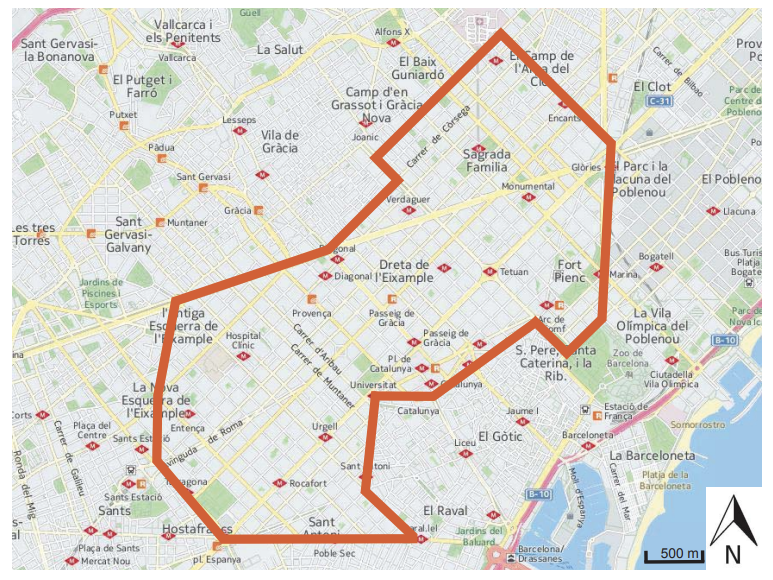
\includegraphics[width=0.7\linewidth]{images/Map of studied area.png}
    \caption{Studied area in Barcelona, Spain. ({Source: \protect\url{http://maps.here.com}}) }
    \label{fig: barcelona map}
\end{figure}